
\chapter{Resultados Experimentais }
\label{cap:resultados}

\section{Resultados}


\subsection{RC3, RC7 e RC28}

Assim como feito em \cite{greciaLin}, iremos usar dados supostos disponíveis diariamente no chão de fábrica. Portanto, para um lote recém expedido,
não podemos usar os índices RC3 e RC7 para auxiliar na predição de RC28. Dessa maneira, iremos usar os últimos índices RC3 e RC7 disponível para o lote expedido no dia $t$,
i.e. o índice RC3 do dia $t-3$ e RC7 do dia $t-7$, que acabaram de ser medidos. \\


\subsection{Abordagem Não-Temporal}

 Para ambos as classes de modelos os dados foram transformados para possuirem variância
unitária e média 0. Os índices RC3 e RC7 foram usados como entrada e o índice
RC28 foi usado como saída. Os dados foram divididos em
\textit{treino}, \textit{validação}. Usamos os dados de treino 
para treinar os
modelos, e os de validação apenas para avaliar o seu erro. O Gráfico
~\ref{fig:divrc28} mostram essa divisão. Lembramos que apenas os dados de
validação são inéditos para os modelos, com eles avaliamos a capacidade de
generalização dos modelos. 


\begin{figure}[H]
  \centering
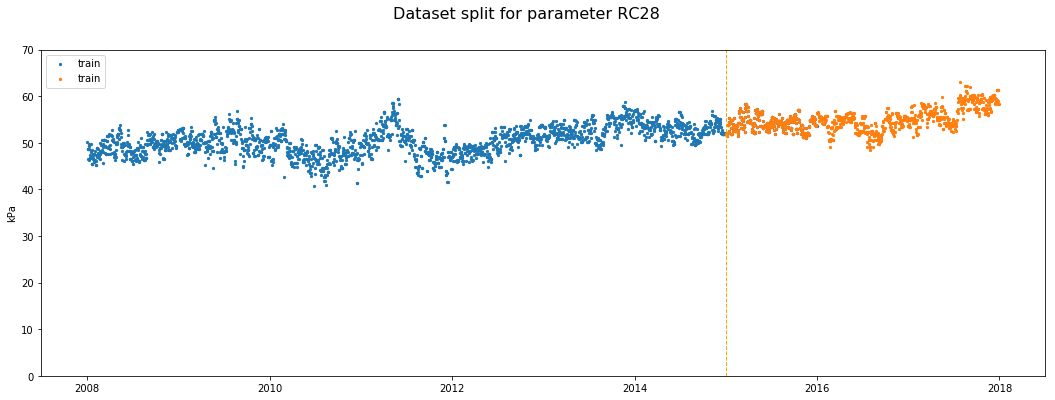
\includegraphics[width=0.9\columnwidth]{split_2008-2015-2017RC28.png}
\caption{Divisão do dataset para a saída RC28, os pontos azuis foram usados para
treino e os pontos laranjas usados para validação.}
  \label{fig:divrc28}
\end{figure}


\subsection{Modelos Bayesianos para Séries Temporais}


Todos os modelos foram implementados usando a bibliteca Pytorch \cite{pytorch}, para os Processos Gaussianos usamos a biblioteca GPyTorch \cite{gpytorch}. Para as predições de séries temporais, usamos todas as entradas de 01/2007 até 09/2018 como nossos dados de treino, e os últimos 3 meses de dados como os dados de validação. As tuplas de treino são da forma $(RC28_{t},\{\})$. Os dados são normalizados pelo método min-max para igualarmos suas grandezas. 




% Local Variables:
% TeX-master: "../quali"
% End:
